\documentclass[sigconf,anonymous,balance=false]{acmart}
\usepackage{array}
% Balance the final bibliography page without changing ACM page geometry.
\usepackage{flushend}

% Add the review option above to display reviewer line numbers.
% Keep anonymous for the double-blind submission.
% This is a writing template: replace all Writing guide paragraphs.
% Keep natural paragraph spacing at zero; distribute flushbottom stretch
% across ordinary prose boundaries rather than heading-before glue alone.
\newcommand{\bodypar}{\par\vskip 0pt plus 6pt\relax}
\newcommand{\writingguide}[1]{\par\noindent\textit{Writing guide: #1}\par}

% Anonymous FPGA '27 draft: retain ACM's reference block and conference footer.
% Do not claim a publication license or use unassigned DOI/ISBN placeholders.
% Replace the rights and publication metadata with ACM's eRights values
% when preparing the accepted paper.
\setcopyright{none}
\settopmatter{printacmref=true,printccs=true,printfolios=true}
\acmDOI{}
\acmISBN{}
% Public conference information for the draft header, from the FPGA'27 CFP.
% Replace publication metadata with ACM's supplied values after acceptance.
\acmConference[FPGA '27]{35th ACM/SIGDA International Symposium on Field-Programmable Gate Arrays}{March 14--16, 2027}{California, USA}
\acmYear{2027}
% Copyright metadata will be supplied by ACM eRights after acceptance.
% Leave the draft copyright year empty to avoid printing an isolated year.
\copyrightyear{}

\title[FHEStore: A Framework for FHE Input Preparation]{FHEStore: An FPGA-based Computational Storage Framework for Input Preparation in Fully Homomorphic Encryption}

% Author and affiliation fields are intentionally omitted during review.
% For the accepted version, remove anonymous and add real author metadata.
% Add the publication metadata supplied by ACM only after acceptance.
% \author{Author name}
% \affiliation{\institution{Institution}\city{City}\country{Country}}
% \email{author@example.org}
% \acmSubmissionID{ID supplied by the submission system}

\begin{document}

\begin{abstract}
Fully homomorphic encryption (FHE) accelerators speed up privacy-preserving computation on encrypted data, serving as ciphertext consumers, while the host conventionally acts as the producer. For applications over persistent data, the conventional host path loads stored data into host memory for encoding, encryption, and ciphertext organization. As homomorphic computation is accelerated, this input preparation accounts for a larger share of workflow latency. Encryption also expands application values into larger ciphertexts, increasing buffering requirements and data movement within this preparation stage.

We present FHEStore, an FPGA-based computational storage framework for FHE input preparation. We develop a high-level synthesis (HLS) operator that integrates radix encoding with Fast Fully Homomorphic Encryption over the Torus (TFHE) encryption. Each generated mask coefficient feeds both dot-product accumulation and incremental ciphertext output, avoiding buffering a complete mask vector. We further propose an operator stream composition method that accounts for ciphertext expansion. It connects optional preprocessing to encryption, determines ciphertext buffer capacity from the value count and ciphertext representation, and coordinates the composed operators through stream flow control.

\begingroup
\emergencystretch=1em
We implement FHEStore and evaluate it against host CPU baselines. With 1~KiB of plaintext input, the encryption operator achieves a $5.00\times$ speedup, while input preparation achieves a $2.45\times$ speedup. The evaluation also shows lower cumulative host CPU time and peak host memory.
\par\endgroup
\end{abstract}

% Draft CCS selections. Generate the matching CCSXML through ACM's CCS
% tool before preparing the submission metadata.
\ccsdesc[500]{Hardware~Hardware accelerators}
\ccsdesc[500]{Information systems~Storage architectures}
\ccsdesc[500]{Security and privacy~Cryptography}
\keywords{Fully Homomorphic Encryption, TFHE, FPGA, High-Level Synthesis, Computational Storage, Streaming Dataflow}

% Allow the longer title in the ACM reference block to break within the column.
\emergencystretch=1em
\maketitle
\emergencystretch=0pt

\section{Introduction}
\label{sec:introduction}

\begin{figure}[!t]
  \centering
  % Exported directly from input-preparation-motivation-v5/input-preparation-motivation.svg.
  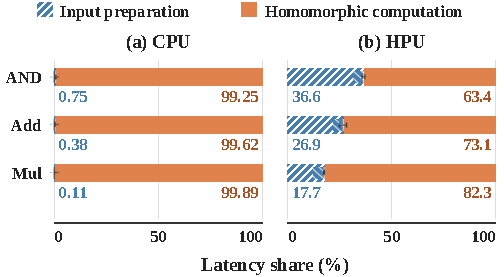
\includegraphics[width=\columnwidth]{figures/input-preparation-motivation-v5/input-preparation-motivation.pdf}
  \caption{Latency shares with (a) CPU and (b) HPU homomorphic computation.}
  \label{fig:preparation-motivation}
  \Description{Two side-by-side panels of thin horizontal stacked bars compare bitwise AND, addition, and multiplication, labeled AND, Add, and Mul. Each bar displays the mean shares of both input preparation and homomorphic computation. With the same host CPU input preparation, its share of preparation plus computation latency ranges from 0.11 to 0.75 percent for CPU homomorphic computation and from 17.7 to 36.6 percent for HPU homomorphic computation.}
\end{figure}

Fully homomorphic encryption (FHE) enables a data owner to outsource computation over encrypted data without revealing the plaintext to the evaluator~\cite{gentry2009fhe}. Hardware accelerators improve homomorphic computation through specialized arithmetic and memory-aware architectures~\cite{xu2026hera,zhou2023fhemem,vanbeirendonck2023fpt,kim2022bts,kim2022ark,samardzic2021f1,samardzic2022craterlake}. These accelerators act as ciphertext consumers. For applications over persistent data, the host conventionally serves as the producer, coordinating data access, encoding, encryption, and ciphertext organization. This FHE input preparation supplies ciphertexts to the consumer, so application performance depends on both stages.
\bodypar

Figure~\ref{fig:preparation-motivation} compares bitwise AND, addition, and multiplication on a CPU and Zama's open-source FPGA-based homomorphic processing unit (HPU)~\cite{zama2025hpu}. Both workflows use the same host CPU input preparation: SSD reads, encoding, and encryption, ending with ciphertexts in host memory. Only homomorphic computation changes from CPU software to HPU acceleration. Shares are normalized to preparation plus computation latency, excluding network transfer; bars show means, and error bars span the observed minimum and maximum. Input preparation accounts for 0.11\%--0.75\% with CPU execution and 17.7\%--36.6\% with HPU acceleration, making host-side input preparation an increasingly important optimization target.
\bodypar

Host-side input preparation couples cryptographic computation with data access and ciphertext organization. Encoding and encryption consume CPU resources, while input batches and expanded ciphertexts occupy host memory. Optional preprocessing, such as record selection, can exclude unneeded data before encryption, reducing cryptographic computation and ciphertext movement. Accelerating input preparation requires coordinating data access and ciphertext buffering with encoding and encryption.
\bodypar

Encryption accelerators optimize cryptographic arithmetic and parallel execution~\cite{mert2020bfv,lee2023ckks,feryputri2025lwe,syafalni2026multicore}. Client-side and end-to-end systems further coordinate cryptographic processing with encoding, memory organization, or communication~\cite{krieger2024aloha,yune2025abcfhe,vanderhagen2022choco,gupta2024memfhe}. For persistent-data applications, input preparation also encompasses storage access and optional preprocessing. Placing encoding and encryption alongside storage access connects device-local input, operator streams, and ciphertext output in one execution path.
\bodypar

We present FHEStore, an FPGA-based computational storage framework for FHE input preparation. A computational storage device (CSD) places programmable processing alongside storage access~\cite{snia2025csmodel,ruan2019insider,wong2024dongle,woods2014ibex}. Using high-level synthesis (HLS), FHEStore implements radix encoding and Fast Fully Homomorphic Encryption over the Torus (TFHE)~\cite{chillotti2020tfhe} encryption in an encryption operator, a streaming FPGA processing module. A stream switch connects operators and directs ciphertext output to device-local buffers. An operator context holds task-specific parameters; task control installs these contexts and binds stream connections and memory ranges. The host coordinates execution and retrieves the completed ciphertexts.
\bodypar

\begingroup
\setlength{\leftmargini}{1.2em}
\setlength{\listisep}{2pt}
\setlength{\partopsep}{0pt}
\setlength{\itemsep}{2pt}
\setlength{\parsep}{0pt}
We make the following contributions:
\begin{itemize}
  \item \textbf{Integrated HLS operator for TFHE encoding and encryption.} A TFHE encryption operator integrates radix encoding and encryption, traversing the mask once per learning-with-errors (LWE) block. Each coefficient feeds dot-product accumulation and incremental ciphertext output without buffering a complete mask vector.
  \item \textbf{Operator stream composition accounting for ciphertext expansion.} A method connects optional preprocessing to encryption, determines ciphertext buffer capacity from the value count and ciphertext representation, and coordinates the composed operators through stream flow control.
  \item \textbf{Prototype implementation and evaluation.} We implement and evaluate an FHEStore prototype (Section~\ref{sec:evaluation}). With 1~KiB of plaintext input, the encryption operator and input preparation achieve $5.00\times$ and $2.45\times$ speedups over host CPU baselines, respectively, with lower cumulative host CPU time and peak host memory.
\end{itemize}
\endgroup

% Queue the architecture early to retain its placement at the top of page 3.
\begin{figure*}[t]
  \centering
  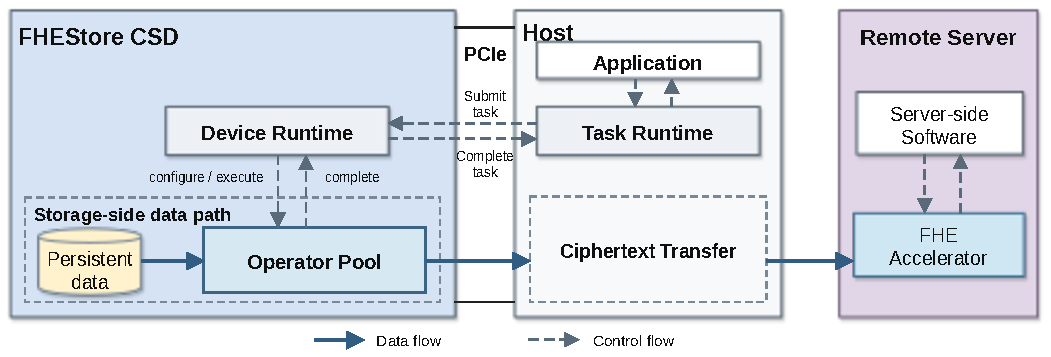
\includegraphics[width=\textwidth]{figures/fhestore-overview-v8/fhestore-overview.pdf}
  \caption{FHEStore architecture for FHE input preparation. Solid blue arrows denote data flow; dashed gray arrows denote control flow.}
  \Description{Persistent data feed the CSD operator pool. The device runtime configures the pool and receives execution completion. The host application interacts with the task runtime, which submits tasks to the device runtime and receives completion notifications over PCIe. Ciphertext transfer retrieves generated ciphertexts from the CSD over PCIe into host memory. The host then forwards them over the network to the remote server. The remote server contains server-side software and an FHE accelerator.}
  \label{fig:pipeline}
\end{figure*}

\section{Background}
\label{sec:background}
\subsection{FHE and TFHE Fundamentals}
FHE enables computation on encrypted data without revealing the underlying plaintext to the evaluator~\cite{gentry2009fhe}. It provides key generation, encryption, homomorphic evaluation, and decryption. TFHE is a lattice-based FHE scheme over the torus $\mathbb{T}=\mathbb{R}/\mathbb{Z}$, where the period is normalized to one~\cite{chillotti2020tfhe}.
\bodypar

Encoding maps application values into the scheme's message representation; decoding maps decrypted messages back into application values. Let $k_{\mathrm{enc}}$, $k_{\mathrm{dec}}$, and $k_{\mathrm{eval}}$ denote the encryption, decryption, and evaluation key material. For messages $m_1,\ldots,m_t$, form $c_i\leftarrow\operatorname{Enc}_{k_{\mathrm{enc}}}(m_i)$. Evaluation applies $f$ to these ciphertexts using $k_{\mathrm{eval}}$ to obtain $c_f$. With valid parameters, an exact scheme satisfies the following relation for a supported computation $f$, with overwhelming probability over its randomness:
\begin{equation}
  \operatorname{Dec}_{k_{\mathrm{dec}}}(c_f)=f(m_1,\ldots,m_t).
  \label{eq:fhe-correctness}
\end{equation}
\bodypar

LWE describes noisy linear equations modulo an integer, providing a basis for lattice-based cryptography~\cite{regev2009lwe}. TFHE uses LWE and ring learning-with-errors (RLWE) ciphertexts, with bootstrapping to control noise~\cite{chillotti2020tfhe}. For secret-key torus-LWE encryption, let $\mu=\operatorname{Encode}(m)$ belong to a discrete message space $\mathcal{M}\subset\mathbb{T}$, and let $\mathbf{s}\in\mathbb{Z}^{n}$ be the secret key. Sampling a uniform mask $\mathbf{a}\in\mathbb{T}^{n}$ and an error $e$ from the scheme's noise distribution yields
\begin{equation}
  c=(\mathbf{a},b),\qquad
  b=\langle\mathbf{a},\mathbf{s}\rangle+\mu+e\;(\mathrm{mod}\,1).
  \label{eq:torus-lwe-encryption}
\end{equation}
Decryption computes the phase,
\begin{equation}
  \phi_{\mathbf{s}}(c)=b-\langle\mathbf{a},\mathbf{s}\rangle
  =\mu+e\;(\mathrm{mod}\,1),
  \label{eq:torus-lwe-phase}
\end{equation}
and recovers the encoded message when the phase remains within its decision region~\cite{chillotti2020tfhe}.
\bodypar

A finite-precision representation stores each torus coefficient as a $q$-bit integer corresponding to a multiple of $2^{-q}$. Torus addition then becomes integer addition modulo $2^q$. This representation connects the encryption equation to coefficient arithmetic in hardware.
\bodypar

For integer inputs, radix encoding decomposes each application value into fixed-width digits. Each digit is encoded as a torus message and encrypted as an LWE block; the ordered blocks form a ciphertext bundle representing that value. Each block contains $n+1$ coefficients, so the bundle's size depends on the digit count, LWE dimension, and coefficient precision. The value count and ciphertext bundle size determine the ciphertext buffer capacity and transfer volume required during input preparation.

\subsection{FHE Producer--Consumer Workflows}
Outsourced FHE systems place input preparation in the data owner's trusted domain and homomorphic computation at an external consumer~\cite{krieger2024aloha,yune2025abcfhe,gupta2024memfhe}. The producer coordinates data access, encoding, encryption, and ciphertext organization. The consumer executes the encrypted program using ciphertexts and evaluation material; the secret key remains in the trusted domain.
\bodypar

Client-side accelerators connect encoding and encryption to software control and memory transfers~\cite{krieger2024aloha,yune2025abcfhe}, while FHE accelerators schedule encrypted operations over ciphertexts and evaluation keys in their memory systems~\cite{xu2026hera,zhou2023fhemem,vanbeirendonck2023fpt}. Producer and consumer must agree on cryptographic parameters, message encoding, and ciphertext layout. Client-side systems coordinate local processing with encrypted computation across this interface~\cite{vanderhagen2022choco}.

\subsection{Computational Storage and Application Integration}
Computational storage couples processing with storage to offload host work or reduce data movement~\cite{snia2025csmodel}. Operations such as filtering, aggregation, feature selection, and decompression transform data along the storage-access path~\cite{ruan2019insider}. Their output representation affects the benefit: filtering can shrink the returned data, while encryption expands it.
\bodypar

FPGA storage frameworks expose data access and processing through virtual files, C++ data and parameter streams, and unified HLS interfaces for memory and storage~\cite{ruan2019insider,wong2024dongle}. These abstractions express task parameters and input and output locations while the framework coordinates transfers and completion. FHEStore integrates encryption with this storage-side execution model (Section~\ref{sec:architecture}).

\section{System Overview}
\label{sec:architecture}

\subsection{System Organization}
\label{subsec:system-organization}

\begingroup
\emergencystretch=1em
FHEStore organizes input preparation across a CSD and host software connected over PCIe (Figure~\ref{fig:pipeline}). The CSD combines persistent storage, device-local buffers in Subsystem Local Memory (SLM)~\cite{nvme2025slm}, and an FPGA operator pool. The remote server represents an external privacy-preserving outsourcing service equipped with an FHE accelerator.
\par
\endgroup
\bodypar

Persistent data enter device-local buffers and feed an operator graph whose modules exchange records or values through streams. Optional preprocessing supplies application values to the encryption operator, which integrates encoding with encryption. Generated ciphertexts are collected in device-local output buffers.
\bodypar

The host task runtime interprets application requests, while the device runtime binds them to the CSD's operators and memory resources. Control messages submit an execution program describing operator requirements and stream connections, together with operator contexts, then report completion. Ciphertext transfer retrieves the output SLM range into host memory over PCIe and identifies the ciphertext sequence using the reported valid ciphertext length. The host can then forward the sequence over the network to the external consumer.
\bodypar

As in Section~\ref{sec:background}, the host and CSD belong to the data owner's trusted domain, where plaintext processing and key-dependent encryption occur. The host resolves locally held key material and supplies the LWE secret key $\mathbf{s}$ through the encryption operator's context when preparing execution. The external consumer receives ciphertexts, while local task control retains their association with the source data.

\subsection{Application Task Model}
\label{subsec:application-task}

An application specifies input preparation through a task $T=(D,Q,E,O)$. $D$ identifies the stored input and its layout, $Q$ specifies optional preprocessing, $E$ selects the encoding and cryptographic configuration, and $O$ identifies the output location in host memory. The task runtime checks these descriptions before submitting device execution.
\bodypar

The input description combines a storage range with its content interpretation. With $Q$ omitted, packed application values enter encryption directly in source order; otherwise, preprocessing supplies the values to encrypt. Both forms define an ordered sequence $x_0,\ldots,x_{M-1}$ of $M$ application values. With configuration $E$ and secret key $\mathbf{s}$, the task produces
\begin{equation}
  c_j \leftarrow \operatorname{Enc}_{\mathbf{s},E}\!\left(
    \operatorname{Encode}_{E}\!\left(x_j\right)
  \right),\quad 0\leq j<M.
  \label{eq:task-ciphertexts}
\end{equation}
Here, $c_j$ is the ciphertext bundle representing $x_j$ under $E$, including multiple ciphertexts when required by the encoding. The task returns the ordered ciphertext sequence at $O$, independently of the device resources used.
\bodypar

Selection and projection provide one case of optional preprocessing. For source records $r_0,\ldots,r_{N-1}$, the schema in $D$ identifies record boundaries, field types, and offsets. Selection evaluates the predicates in $Q$, and projection chooses the field passed to encryption. Let $\mathcal{I}_Q=(i_0,\ldots,i_{M-1})$ list the selected indices in source order and $\pi_Q$ denote the field projection. Equation~\eqref{eq:task-ciphertexts} then uses $x_j=\pi_Q(r_{i_j})$.

For a selective task, the host retains the source-record mapping $\mathcal{I}_Q$ derived from the selection manifest, which records source-record identities and selection results. This mapping associates each ciphertext bundle with its source record, including records with identical projected values. An empty selection yields an empty ciphertext sequence and mapping.

\subsection{Operator Graphs and Device Execution}
\label{subsec:operator-execution}

The task runtime translates $T$ into an operator graph, operator contexts, and input and output SLM ranges. Graph nodes identify operator functions, and edges specify the streams exchanged between their ports. An execution program records the graph's operator requirements, connections, and entry and terminal endpoints for submission to the device runtime. Keeping these objects distinct connects application semantics to device execution: the graph defines the computation, contexts supply its task-specific interpretation, and SLM ranges identify the data it consumes and produces.
\bodypar

Operator contexts carry the input interpretation from $D$, optional preprocessing settings from $Q$, and the encryption configuration from $E$. The encryption operator's context also contains its locally supplied key material. Contexts bind task-specific parameters to the graph's logical operators. For a selective task, the operator context for preprocessing determines which fields are inspected and which field is emitted, while the operator context for encryption determines how each emitted value becomes a ciphertext bundle. Section~\ref{sec:implementation} develops the encryption operator's internal design.
\bodypar

An input SLM range identifies the device-local input buffer, its offset, and its byte extent. An output SLM range identifies the destination buffer and the extent available for ciphertext reception. These ranges bind graph endpoints to data locations without encoding those locations into the operator's processing logic. Their extents also distinguish the bounded input consumed by an execution from the capacity reserved for its expanded output. The device runtime receives the range bindings together with the execution program and operator contexts.
\bodypar

Before execution, the device runtime assigns the graph to available operators, installs their contexts, and binds stream destinations through the stream switch. The graph's logical connections determine the downstream operator or output endpoint for each stream. A task without preprocessing uses the encryption operator alone; a selective task connects preprocessing to encryption. Connected operators exchange values through the operator interconnect during device execution.

Device completion reports the valid ciphertext length in the output SLM range after the graph finishes, separately from allocated capacity and execution framing. The task runtime passes this length to ciphertext transfer. Application completion denotes availability at $O$ in host memory, with the source-record mapping retained for selective tasks. Section~\ref{sec:production} develops the operator stream composition method, including stream routing and ciphertext buffer allocation.
\section{HLS Design of TFHE Encoding and Encryption}
\label{sec:implementation}

FHEStore's HLS encryption operator receives ordered application values and generates their ciphertext bundles. Figure~\ref{fig:tfhe-encryption} organizes the datapath into input and context, sampling, encryption arithmetic, and packetization, connecting the torus-LWE operation in Section~\ref{sec:background} to the storage-side stream in Section~\ref{sec:architecture}. Encoding and encryption share one invocation: radix digits become LWE blocks within the datapath, while coefficients leave incrementally through the packetizer.

\begin{figure*}[t]
  \centering
  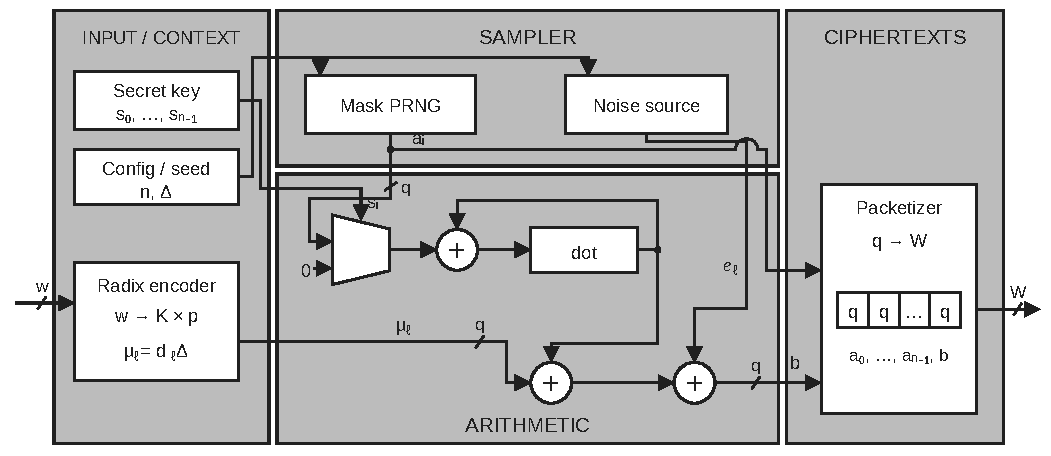
\includegraphics[width=\textwidth]{figures/tfhe-encryption-v4/tfhe-encryption.pdf}
  \caption{HLS architecture for integrated TFHE encoding and encryption.}
  \Description{Four functional regions contain input and context, mask and noise sampling, encryption arithmetic, and ciphertext packing. The radix encoder takes w-bit application values. A binary-key selector feeds a dot-product accumulator with feedback. Two additions combine the dot product, encoded digit, and noise. Mask coefficients and the body feed the packetizer, which outputs W-bit ciphertext beats.}
  \label{fig:tfhe-encryption}
\end{figure*}

\subsection{Representation and Streaming Interface}
\label{subsec:tfhe-interface}

Let $w$ denote the application-value width, $p$ the message bits per radix digit, and $K=\lceil w/p\rceil$ the number of digits representing a value. Each digit produces one LWE block with $n$ mask coefficients and a body. Thus, a ciphertext bundle contains $K$ blocks, ordered from the least-significant digit to the most-significant digit. Torus coefficients have width $q$, while the physical stream has width $W$. A beat is one transfer on this stream interface. The packetizer places $L=W/q$ coefficients in a ciphertext beat, with $q$ dividing $W$. Widths and radix counts describe the synthesized datapath; the operator context provides the configuration for a particular execution.
\bodypar

The CPU coefficient layout serializes each block in natural order as $(a_0,\ldots,a_{n-1},b)$. This order gives a direct relationship between the mask index, key index, and output position. The arithmetic uses unsigned coefficients modulo $2^q$, implementing the finite-precision form of torus addition in Equation~\eqref{eq:torus-lwe-encryption}. The binary secret key contains $n$ bits, with $s_i\in\{0,1\}$. Consequently, multiplication by a key coefficient becomes selection of $a_i$ or zero, followed by modular addition.
\bodypar

Both physical ports use AXI4-Stream. The input adapter interprets application-value framing; the packetizer constructs ciphertext beats. Configuration and the bit-packed secret key arrive through the operator context stored in BRAM. Configuration includes the input mode, input count, and pseudorandom number generator (PRNG) seed and nonce. Key indexing selects a context word and a bit within that word. The same key supplies successive blocks, while the coefficient index restarts at each block boundary. The encryption operator reads execution configuration before consuming its first payload beat. The input count controls application-value consumption, whereas coefficient and digit counters control block generation; these counts remain separate as encryption expands each accepted value into a bundle.

Each block's $n+1$ coefficients occupy $\lceil(n+1)/L\rceil$ ciphertext beats, including padding in unused positions. The serialized ciphertext bundle size in bytes is
\begin{equation}
  C=K\left\lceil\frac{n+1}{L}\right\rceil\frac{W}{8}.
  \label{eq:tfhe-bundle-size}
\end{equation}
Block padding belongs to this representation; a separate terminal beat follows the payload and carries completion metadata.

\subsection{Integrated Encoding and Encryption}
\label{subsec:tfhe-encryption}

\begingroup
\emergencystretch=1em
The input adapter supplies one application value $x$ to the radix encoder at a time. Packed mode carries consecutive values within a physical stream beat. The adapter inspects the AXI4-Stream byte-enable mask, TKEEP, and extracts the valid values in stream order. A configured input count bounds consumption when the final physical beat contains additional data. The adapter retains the received beat while its values are processed, allowing the encryption core to operate on a narrower value interface than the external stream.
\par
\endgroup
\bodypar

Scalar mode instead assigns one application value to each payload beat, using its low $w$ bits. This framing matches a preprocessing operator that emits one projected field per selected record. Here, the beat itself identifies one value; the byte-enable mask does not specify a collection of packed inputs. Both modes present the same value interface to the encoder, so the subsequent ciphertext bundle has the same digit and coefficient order.

For an unsigned $w$-bit value $x$, the radix encoder extracts digits and maps them to integer-torus messages:
\begin{equation}
  \begin{aligned}
    d_\ell &= \left\lfloor x/2^{p\ell}\right\rfloor \bmod 2^p,\quad 0\leq\ell<K,\\
    \mu_\ell &= d_\ell\Delta.
  \end{aligned}
  \label{eq:tfhe-radix-encoding}
\end{equation}
The encoding interval $\Delta$ places each digit within the message space represented by a coefficient. With a power-of-two interval, encoding consists of a shift into the corresponding coefficient positions. In this representation, the highest digit carries the remaining high-order bits when $p$ does not divide $w$. The encoder produces each $\mu_\ell$ inside the operator, without materializing an intermediate array of encoded torus messages.

The $K$ digits reuse one encryption core sequentially. The core completes a block and its serialization before advancing to the next digit, and completes the bundle before accepting another value from the input adapter. Value and digit indices establish a ciphertext index for the mask PRNG, while the mask-coefficient index establishes the key position. This nested execution preserves the application-value order across both input modes and the least-significant-first order within each bundle.

\subsection{Coefficient Arithmetic and State}
\label{subsec:tfhe-coefficient-arithmetic}

The arithmetic core traverses each block's mask once. At coefficient index $i$, the PRNG generates $a_i$ and the key reader supplies $s_i$. The same coefficient feeds the packetizer and binary-key selector, whose contribution updates the accumulator:
\begin{equation}
  u_{i+1}=(u_i+s_i a_i)\bmod 2^q,\qquad u_0=0.
  \label{eq:tfhe-encryption-accumulation}
\end{equation}
After the traversal, the body $(u_n+\mu_\ell+e_\ell)\bmod 2^q$ follows the mask into the packetizer. Figure~\ref{fig:tfhe-encryption} shows the additions combining the dot product, digit, and noise.

The mask PRNG initializes its state from the context's seed and nonce and the ciphertext index. After mask generation, the noise source uses the same generator to obtain a bounded magnitude and sign for $e_\ell$.
\bodypar

Incremental emission avoids retaining a complete mask vector before serialization. The datapath holds generator state, the dot-product accumulator, coefficient and digit indices, and a partially filled ciphertext beat; the packed key remains in the context. Conditional modular addition updates the accumulator, and body additions follow the completed recurrence. The $W$-bit output interface combines consecutive coefficients into a beat, while the arithmetic core generates those coefficients sequentially.

\subsection{Ciphertext Packetization and Completion}
\label{subsec:tfhe-packetization}

The packetizer maintains a $W$-bit register and a count of occupied coefficient positions. Each arriving mask coefficient fills the next position. A full register is emitted as a ciphertext beat, after which the register and position count reset. The body follows the mask in the same sequence and forces a flush, even when fewer than $L$ coefficient positions are occupied. Unused positions remain zero. The following LWE block starts in a fresh beat, preserving a block stride of $\lceil(n+1)/L\rceil$ beats and making block boundaries independent of input framing.
\bodypar

AXI4-Stream ready/valid flow control connects packetization to the surrounding data path. A blocked output write holds the pending beat and stalls progression through the coefficient traversal. The retained arithmetic and packet state preserve the relationship between generated coefficients, their accumulated contributions, and their output positions. The input adapter consequently waits while the core finishes the current ciphertext bundle.

The operator accepts a fixed input count or a stream whose length is determined by an upstream terminal beat. With a fixed count, it encrypts the requested values and waits for the terminal beat; a premature terminal beat identifies an incomplete input. The terminal beat follows all ciphertext payload and carries completion metadata separately. Payload beats remain data beats regardless of a block boundary. Separating the terminal beat from block padding lets the receive path derive the valid ciphertext length and report device completion after ciphertext reception.
\section{Storage-Side FHE Input Preparation}
\label{sec:production}

FHEStore's operator stream composition method connects optional preprocessing to encryption while accounting for ciphertext expansion. It combines stream routing with ciphertext buffer allocation and stream flow control. Figure~\ref{fig:ciphertext-production} shows the operator interconnect through which the composed operators exchange data.

\subsection{Operator Stream Composition}
\label{subsec:streaming-production}

The device runtime first loads the task's SSD range into its input SLM range. Once loading completes, the read DMA supplies this range as an AXI4-Stream to the graph's entry. The write DMA receives the final stream into an output SLM range, collecting ciphertexts as encryption produces them.
\bodypar

Memory binding and stream routing determine different parts of this path. DMA descriptors specify the buffer addresses and byte extents accessed at the memory endpoints. Destination tags identify where a beat travels within the operator graph. An operator-to-operator handoff therefore requires a downstream destination, while the memory endpoint requires a bound range in which to read or write data. This separation lets the same operator graph execute over different bound memory ranges.
\bodypar

The stream switch forwards beats according to the AXI4-Stream destination field, TDEST. Figure~\ref{fig:ciphertext-production} illustrates route composition using slot and port identifiers: the upper and lower fields identify a destination slot and input port. The example route $\{3,1\}$ selects Port~1 of Operator~\#3, while the reserved output route $\{\mathrm{F},2\}$ selects memory-output channel~2. The device runtime's scheduler binds graph edges to their destinations and configures each source operator's next-hop route. Operator controllers attach the resulting destination tag to outgoing beats, while the device runtime programs the read DMA's entry destination. Each operator returns its output to the same stream switch, which forwards it to the next operator or the write DMA.
\bodypar

For packed values, the graph connects read DMA directly to encryption and routes ciphertext bundles to write DMA. Optional preprocessing inserts operators before encryption while retaining the graph's memory endpoints.
\bodypar

For a selective task, the selection and projection operator implements $Q$ from Section~\ref{subsec:application-task}. Its context specifies record layout, predicate-field offsets and types, comparison operands, Boolean expression, and projected field. It captures required fields as record beats arrive and evaluates predicates at record boundaries. These settings can change independently of stream destinations.
\bodypar

During the selective task's encryption pass, each matching record supplies one projected value in source order to the encryption operator's scalar interface (Section~\ref{subsec:tfhe-encryption}). Values pass through the stream switch without an intermediate array in SLM, and ciphertext bundles follow the direct graph's output route.
\bodypar

Ciphertext expansion couples flow control to operator composition: encryption may occupy many output beats for each input value. Input FIFOs absorb short rate differences, while AXI4-Stream backpressure stalls upstream processing when downstream capacity is unavailable. This mechanism coordinates preprocessing, encryption, and ciphertext reception within finite buffers.

\begin{figure}[t]
  \centering
  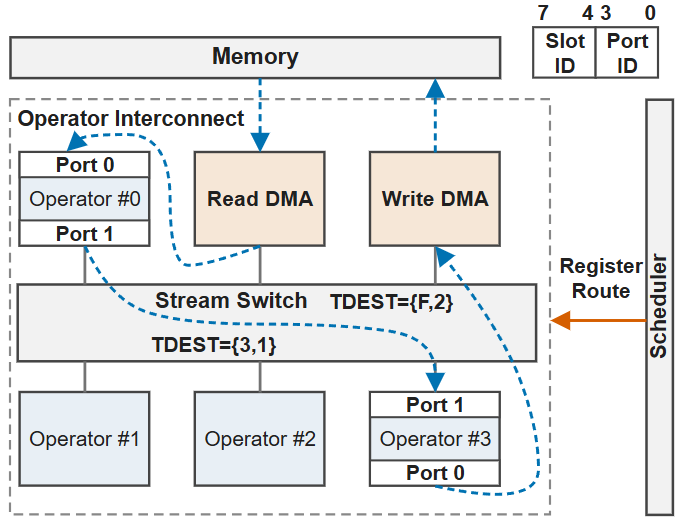
\includegraphics[width=\columnwidth]{figures/ciphertext-production-v4/author-upload.png}
  \caption{Operator interconnect and an example stream route. Dashed blue arrows show data flow.}
  \Description{Memory connects to read and write DMA endpoints above a shared stream switch. Four operator boxes surround the switch. Dashed blue arrows trace an example path from memory through read DMA, operator 0, operator 3, and write DMA back to memory. Destination labels identify the next operator port and the terminal endpoint. A scheduler beside the interconnect indicates route registration, and a field diagram shows slot and port identifiers.}
  \label{fig:ciphertext-production}
\end{figure}

\subsection{Execution and Output Management}
\label{subsec:production-management}

The output SLM range must accommodate the representation produced by the graph. For the $M$ application values defined in Section~\ref{subsec:application-task}, the ciphertext payload occupies $MC$ bytes, where $C$ is the serialized ciphertext bundle size in Equation~\eqref{eq:tfhe-bundle-size}. The output extent therefore depends on both the value count and the encoding configuration. The receive range reserves space for the payload and a terminal beat, rounded to the allocation alignment:
\begin{equation}
  B_{\mathrm{out}}=A\left\lceil\frac{MC+F}{A}\right\rceil,
  \label{eq:production-output-range}
\end{equation}
where $A$ is the allocation alignment and $F$ is the terminal-beat size. Valid ciphertext length is $MC$; terminal-beat and allocation padding bytes belong only to the receive extent. Without selection, $M$ follows from the input count.
\bodypar

Because input framing leaves $C$ unchanged, the task runtime sizes the receive range using $M$ and $C$, independently of intermediate routes.
\bodypar

Execution begins by preparing the write DMA's receive descriptors before starting the read DMA. This ordering makes the bound output range available when the operator graph starts producing ciphertexts. After the payload, the encryption operator emits a separate terminal beat. The device runtime recognizes the terminal beat in receive completion, excludes its bytes from payload accounting, and reports the valid ciphertext length. Device completion identifies the point at which the graph's ciphertext output is available in SLM. Ciphertext transfer retrieves the aligned output range into host memory and identifies the valid ciphertext sequence using the reported length, including serialized block padding and excluding the terminal beat and allocation padding.
\bodypar

For a selective task, FHEStore determines the data-dependent $M$ through a discovery pass over the input SLM range. In this mode, preprocessing produces a selection manifest with an entry for each source record, containing its index, selection flag, and selected projected value, followed by a count summary. The stream switch directs this output to the write DMA and a temporary output SLM range. Its extent is determined by the source-record count, so the selection manifest can be received before the selected count is known. The host retrieves the selection manifest and checks its record identities, selection flags, task metadata, and summary count. It then obtains $M$ and the source-record mapping $\mathcal{I}_Q$.
\bodypar

The task runtime uses $M$ to allocate the ciphertext output SLM range and launches the encryption pass with the operator graph that connects preprocessing to encryption. This pass reads the same input SLM contents and applies the same selection and projection. For $M>0$, the task uses one SSD load and two SLM scans. The selection manifest remains host-side task metadata, and the host associates the retrieved ciphertext bundles with $\mathcal{I}_Q$. If $M=0$, the task skips the encryption pass and returns an empty ciphertext sequence and mapping.
\bodypar

Larger selective tasks use batches with bounded source-record counts, bounding input buffers, manifests, and maximum ciphertext output even when every record matches. Each batch runs the discovery pass, allocates ciphertext buffers, and runs the encryption pass when its selected count is nonzero.
\bodypar

Batches execute sequentially, releasing device buffers after output retrieval. The host adjusts selected indices by each batch's source-record offset, preserving source-record mapping and ciphertext order across batch boundaries.

\section{Experimental Evaluation}
\label{sec:evaluation}
\subsection{Experimental Setup}
We implement FHEStore on a SoC FPGA-based computational storage platform and evaluate FHE input preparation from persistent data. The evaluation covers encryption operator performance, input-preparation performance, host resource consumption, and application-directed preprocessing. The host software path serves as the baseline; figures and tables identify the two paths as CPU baseline and FHEStore.
\bodypar

Table~\ref{tab:experimental-platform} summarizes the platform configuration. The device-side ARM processor runs the management software for SSD access, device memory management, and FPGA task scheduling, while the FPGA programmable logic executes preprocessing and encryption operators. The computational storage client submits tasks to the device and retrieves ciphertexts. It then transfers the ciphertexts over the network to a remote server equipped with a Zama HPU, which performs homomorphic computation.
\bodypar

\begin{table}[!htbp]
  \centering
  \caption{Experimental platform configuration.}
  \label{tab:experimental-platform}
  \small
  \renewcommand{\arraystretch}{1.16}
  \begin{tabular}{@{}p{0.30\columnwidth}>{\raggedright\arraybackslash}p{\dimexpr0.70\columnwidth-2\tabcolsep\relax}@{}}
    \toprule
    \textbf{Component} & \textbf{Configuration} \\
    \midrule
    Host CPU & Intel Xeon Gold 6248R \\
    Host memory & 256~GB DDR4 \\
    Host kernel & Linux 5.15.135-yfl \\
    SoC FPGA platform & Fidus Sidewinder-100 with Zynq UltraScale+ XCZU19EG \\
    Device processor & Quad-core ARM Cortex-A53 \\
    Device memory & 16~GB \\
    Device kernel & Linux 5.4.0 \\
    Persistent storage & NVMe SSD, SSSTC CA5-8D512x1, 512~GB \\
    QEMU & KVM acceleration, 4 vCPUs, 16~GiB memory \\
    QEMU guest kernel & Linux 5.4.211 \\
    Remote HPU & Zama HPU on V80 \\
    \bottomrule
  \end{tabular}
\end{table}

The FPGA design is synthesized using Vivado 2020.2, and the encryption operator runs at 250~MHz. Table~\ref{tab:fpga-resources} summarizes FHEStore's FPGA resource usage, covering computational operators, storage access, data movement, interconnects, and control logic, based on the hierarchical synthesis report.
\bodypar

\begin{table}[!htbp]
  \centering
  \caption{FHEStore FPGA resource usage.}
  \label{tab:fpga-resources}
  \small
  \renewcommand{\arraystretch}{1.16}
  \begin{tabular*}{\columnwidth}{@{\extracolsep{\fill}}lrr@{}}
    \toprule
    \textbf{Resource} & \textbf{Used} & \textbf{Utilization} \\
    \midrule
    LUT & 266,538 & 50.99\% \\
    FF & 343,422 & 32.85\% \\
    LUTRAM & 21,750 & 13.49\% \\
    BRAM (36~Kb equivalent) & 577 & 58.64\% \\
    URAM & 58 & 45.31\% \\
    DSP & 10 & 0.51\% \\
    \bottomrule
  \end{tabular*}
\end{table}

The inputs are unsigned 8-bit integers (u8), each represented by four 2-bit radix blocks, with one LWE ciphertext per block. The LWE dimension is 2048, and coefficients are 64 bits wide. The encryption performance comparison uses the same 64-byte-padded ciphertext layout for both paths. Plaintext size is measured in bytes, with one byte per unsigned 8-bit input value.
\bodypar

The HPU experiments cover bitwise OR, bitwise AND, equality, right shift, addition, subtraction, and multiplication. Application-directed input preparation is evaluated using lineitem data generated by TPC-H \texttt{dbgen}~\cite{tpch2022spec} and the public Intel Lab sensor dataset~\cite{bodik2004intellab}, examining the combined execution of record selection, field projection, and encryption.
\bodypar

We evaluate encryption latency, input-preparation latency, cumulative host CPU time, and peak host memory. In all experiments, the host-side programs for both the CPU baseline and FHEStore run in the same KVM-accelerated QEMU guest described in Table~\ref{tab:experimental-platform}. All performance experiments exclude warm-up runs and use ten valid measurements per configuration; reported values are arithmetic means. Correctness is verified against plaintext reference results.
\bodypar

\subsection{Encryption Operator Performance}
This subsection compares encryption-stage performance between the CPU baseline and FHEStore for plaintext sizes of 1--4096 bytes. FHEStore uses fixed-length binary records converted from TPC-H lineitem data as the plaintext source. Each byte is encrypted as an independent 8-bit plaintext integer, without record selection or field projection.
\bodypar

For the hardware-counter-based comparisons, the CPU baseline records encryption-function execution time, while FHEStore's device-task time is obtained by converting hardware-counter cycles using the operator clock frequency and includes stream-interface waiting during task execution. Speedup is defined as
\begin{equation}
  S_b = \frac{T_{\mathrm{host},b}}{T_{\mathrm{FHEStore},b}},
  \label{eq:speedup}
\end{equation}
where $b$ is the plaintext size in bytes. The numerator and denominator are the CPU baseline and FHEStore latencies in Table~\ref{tab:results}, respectively.
\bodypar

% Author confirmed the updated 4096-byte measurement and ten performance runs on 2026-10-08.
\begin{table}[!htbp]
  \centering
  \caption{Encryption latency and speedup of FHEStore over the CPU baseline.}
  \label{tab:results}
  \small
  \renewcommand{\arraystretch}{1.16}
  \setlength{\tabcolsep}{4pt}
  \begin{tabular*}{\columnwidth}{@{\extracolsep{\fill}}crrc@{}}
    \toprule
    \shortstack{\textbf{Plaintext Size}\\(bytes)} & \shortstack{\textbf{CPU baseline}\\(ms)} & \shortstack{\textbf{FHEStore}\\(ms)} & \shortstack{\textbf{Speedup}\\\phantom{(ms)}} \\
    \midrule
    1 & 0.597 & 0.570 & $1.05\times$ \\
    16 & 8.386 & 2.443 & $3.43\times$ \\
    32 & 15.518 & 3.659 & $4.24\times$ \\
    64 & 31.054 & 6.900 & $4.50\times$ \\
    128 & 62.289 & 13.091 & $4.76\times$ \\
    256 & 124.640 & 26.008 & $4.79\times$ \\
    512 & 252.330 & 51.261 & $4.92\times$ \\
    1024 & 507.577 & 101.596 & $5.00\times$ \\
    2048 & 1016.276 & 202.442 & $5.02\times$ \\
    4096 & 2197.291 & 411.879 & $5.33\times$ \\
    \bottomrule
  \end{tabular*}
\end{table}

% Queue the double-column HPU comparison before the column break so that
% it appears on the page containing the corresponding Section 6.3 discussion.
\begin{figure*}[!t]
  \centering
  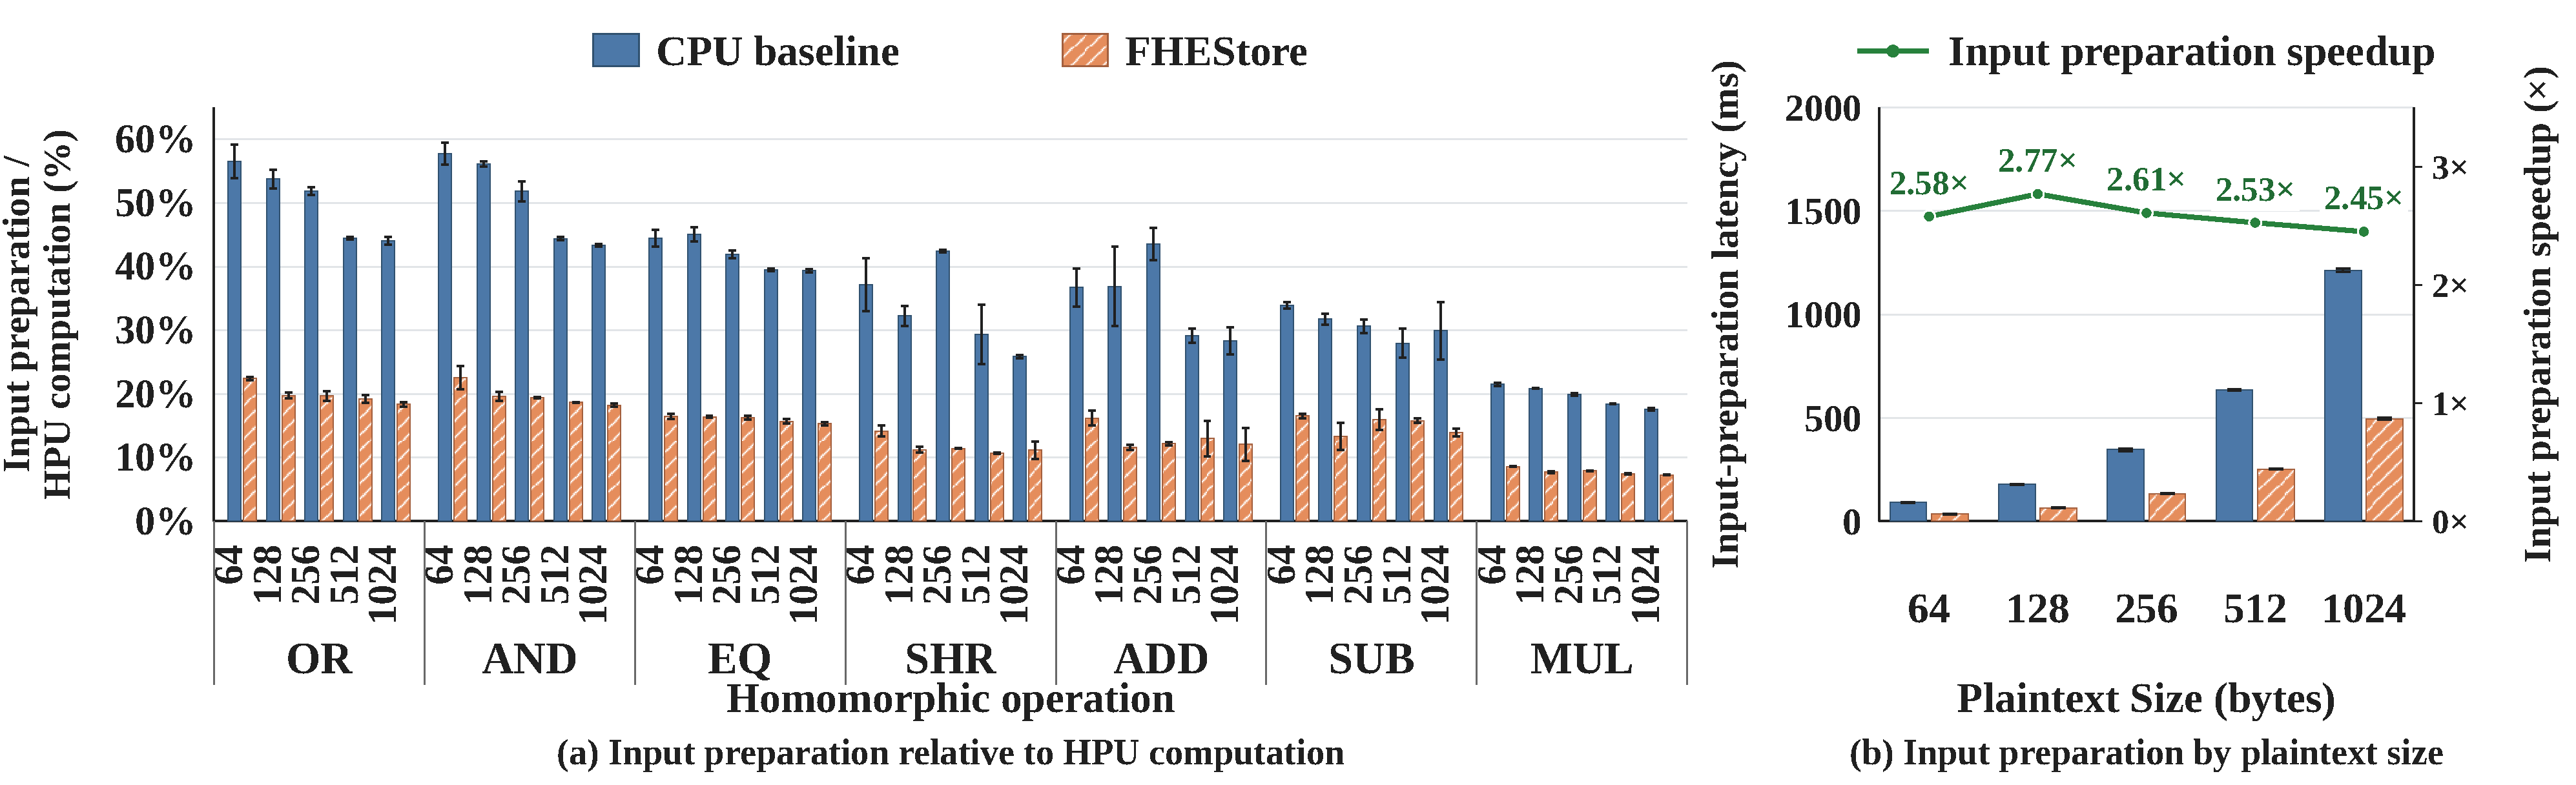
\includegraphics[width=\textwidth]{figures/input-hpu-ratio/input-hpu-two-panels.pdf}
  \caption{Input preparation: (a) latency relative to HPU computation and (b) latency by plaintext size, with speedup on the right axis. Plaintext size is measured per operand. Error bars show (a) run-level sample standard deviations and (b) ranges across seven operations.}
  \Description{The left panel compares CPU baseline and FHEStore input-preparation latency relative to each path's HPU computation latency across seven operations and five plaintext sizes. The right panel compares their preparation latencies averaged equally across seven operations. A green line on the right axis reports CPU baseline latency divided by FHEStore latency: 2.58, 2.77, 2.61, 2.53, and 2.45 times.}
  \label{fig:cpu-hpu-stage-breakdown}
\end{figure*}

Table~\ref{tab:results} reports encryption latency and speedup across plaintext sizes. At 1 byte, the execution times are close, with a speedup of $1.05\times$. FHEStore achieves a $4.76\times$ speedup at 128 bytes. At 2048 bytes, FHEStore reduces encryption latency from the CPU baseline's 1016.276~ms to 202.442~ms, increasing the speedup to $5.02\times$. At 4096 bytes, the speedup reaches $5.33\times$.
\bodypar

\subsection{Input Preparation Performance}
\label{sec:peripheral-overhead}
This subsection compares the cost of preparing ciphertext inputs for the HPU using the CPU baseline and FHEStore. The CPU baseline reads plaintext from the SSD and performs encoding, encryption, and ciphertext organization on the host. FHEStore combines device-side data reads with FPGA encoding and encryption, returning ciphertexts to host memory. Input-preparation latency covers SSD reads, encoding, encryption, ciphertext organization, and required data movement until ciphertexts are available in host memory.
\bodypar

Both paths use the same fixed-length binary records converted from TPC-H lineitem. Plaintext size $B$ is measured in bytes per operand, corresponding to $B$ unsigned 8-bit integers. The first operand uses the first $B$ bytes of the record file; the second adds one to each element modulo 256. The evaluation covers bitwise OR, bitwise AND, equality, right shift, addition, subtraction, and multiplication at plaintext sizes of 64, 128, 256, 512, and 1024 bytes.
\bodypar

Figure~\ref{fig:cpu-hpu-stage-breakdown} summarizes the stage measurements obtained under the unified-input evaluation setup described above. Panel~(a) reports mean input-preparation latency relative to the mean HPU computation latency measured for the corresponding path, including completion synchronization. This normalization characterizes preparation overhead relative to downstream homomorphic computation within each path; error bars show the sample standard deviation of run-level ratios. Panel~(b) directly compares input-preparation latencies: bars show the arithmetic mean of the seven operation-specific mean latencies, and error bars indicate their min--max range. The green line uses the right axis to report input-preparation speedup, defined as CPU baseline mean preparation latency divided by FHEStore mean preparation latency.
\bodypar

Input preparation amounts to 17.58\%--57.73\% of HPU computation latency for the CPU baseline and 7.29\%--22.57\% for FHEStore. For bitwise AND at a plaintext size of 64 bytes, the ratio decreases from 57.73\% to 22.57\%, indicating a substantial relative cost of input preparation for operations with short computation times. Different HPU computation latencies also produce different bar heights at the same plaintext size.
\bodypar

Input-preparation speedups range from $2.45\times$ to $2.77\times$. At a plaintext size of 1024 bytes, mean preparation latency decreases from the CPU baseline's 1211.67~ms to 494.50~ms for FHEStore, yielding a $2.45\times$ speedup. These measurements illustrate the benefit of connecting data access, encoding, and encryption on the storage side to shorten input preparation.
\bodypar

\subsection{Host Resource Consumption}
\label{sec:host-resources}
This subsection examines how storage-side input preparation affects host CPU work and memory requirements. The CPU baseline performs encoding, encryption, and ciphertext organization on the host, whereas FHEStore generates ciphertexts on the device, with the host submitting tasks and retrieving ciphertexts. Both paths use the same SSD plaintext page and retain the resulting ciphertexts in host memory.
\bodypar

The experiment covers plaintext sizes of 64--4096 bytes and measures cumulative host CPU time and peak host memory over the complete execution of the host application process. Cumulative host CPU time is the sum of user and system CPU time across threads, and peak host memory is the maximum resident set size (RSS). The resource CPU baseline uses four workers, unlike the single-core encryption-stage comparison. Bar heights report means, and error bars show sample standard deviations.
\bodypar

% Resource data: logs/encrypt_resources_qemu4_20261004/{cpu,csd}/resource_summary.csv.
% Both configurations record the same input-page SHA-256. The CPU resource
% baseline uses four workers; these are not the single-core Section 6.2 results.
\bodypar

\begin{figure}[!htbp]
  \centering
  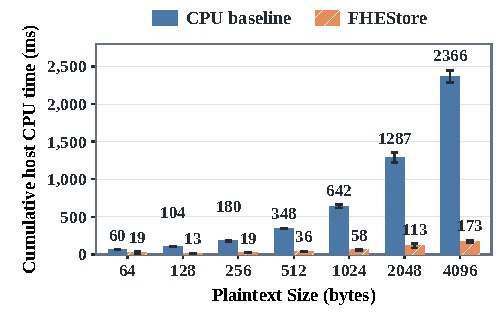
\includegraphics[width=\columnwidth]{figures/host-resources/host-cpu-time.pdf}
  \caption{Cumulative host CPU time for the CPU baseline and FHEStore.}
  \Description{Grouped bars compare cumulative host CPU time for plaintext sizes from 64 to 4096 bytes. FHEStore uses less CPU time at every size. At 2048 bytes, CPU time decreases from 1287.15 to 113.30 milliseconds. Error bars indicate sample standard deviations over ten measurements.}
  \label{fig:host-cpu-time}
\end{figure}

Figure~\ref{fig:host-cpu-time} shows that FHEStore reduces cumulative host CPU time at every measured plaintext size. The reductions reach 91.2\% and 92.7\% at plaintext sizes of 2048 and 4096 bytes, respectively. At 4096 bytes, cumulative host CPU time decreases from 2366.46~ms for the CPU baseline to 172.60~ms for FHEStore. With encoding and encryption performed on the device, the host no longer executes encoding and encryption; its work shifts to task submission, ciphertext retrieval, and related management.
\bodypar

\begin{figure}[!htbp]
  \centering
  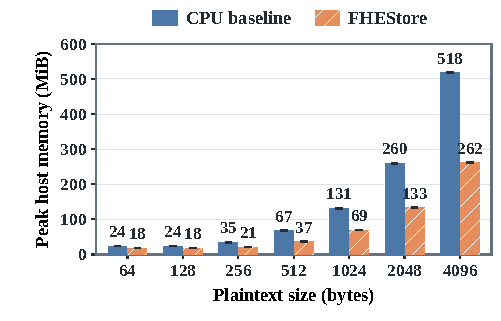
\includegraphics[width=\columnwidth]{figures/host-resources/host-memory.pdf}
  \caption{Peak host memory for the CPU baseline and \mbox{FHEStore}.}
  \Description{Grouped bars compare peak host memory for plaintext sizes from 64 to 4096 bytes. At 2048 bytes, peak memory decreases from 260.09 to 133.14 MiB. At 4096 bytes, it decreases from 517.53 to 261.88 MiB. Error bars indicate sample standard deviations over ten measurements.}
  \label{fig:host-memory}
\end{figure}

Figure~\ref{fig:host-memory} shows the change in peak host memory. At a plaintext size of 2048 bytes, FHEStore reduces peak memory from 260.09~MiB to 133.14~MiB, a 48.8\% reduction; at 4096 bytes, the reduction reaches 49.4\%. Both paths retain output ciphertexts in host memory, while FHEStore's storage-side input preparation reduces the intermediate buffering required for host encoding, encryption, and ciphertext organization.
\bodypar

\subsection{Application-Directed Input Preparation}
\label{sec:selective-generation}
We evaluate FHEStore's ability to configure selection conditions and output fields for application-directed input preparation. The experiments use TPC-H lineitem and Intel Lab sensor data, with 1024 records in each dataset. Each source record is serialized into a fixed-length 512-byte binary layout for device-side preprocessing, with unused positions zero-filled. Table~\ref{tab:application-preprocessing-conditions} lists six preprocessing conditions covering different value ranges, composite predicates, and encrypted output fields.
\bodypar

\begin{table}[!htbp]
  \centering
  \caption{Application-directed preprocessing conditions.}
  \label{tab:application-preprocessing-conditions}
  \small
  \setlength{\tabcolsep}{3pt}
  \renewcommand{\arraystretch}{1.16}
  \begin{tabular}{@{}>{\raggedright\arraybackslash}p{0.06\columnwidth}>{\raggedright\arraybackslash}p{0.62\columnwidth}>{\raggedright\arraybackslash}p{\dimexpr0.32\columnwidth-4\tabcolsep\relax}@{}}
    \toprule
    \textbf{ID} & \textbf{SQL predicate} & \textbf{Encrypted field} \\
    \midrule
    \multicolumn{3}{@{}l}{\textbf{TPC-H}} \\
    C1 & \texttt{WHERE extendedprice\_cents <= }$T_{75}$ & \texttt{quantity} \\
    C2 & \texttt{WHERE extendedprice\_cents <= }$T_{50}$ & \texttt{quantity} \\
    C3 & \texttt{WHERE quantity >= 20}\newline\texttt{AND shipdate < 19950101} & \texttt{shipmode\_code} \\
    \addlinespace
    \multicolumn{3}{@{}l}{\textbf{Intel Lab}} \\
    C4 & \texttt{WHERE humidity\_pct >= }$H_{75}$ & \texttt{humidity\_pct} \\
    C5 & \texttt{WHERE humidity\_pct >= }$H_{50}$ & \texttt{humidity\_pct} \\
    C6 & \texttt{WHERE temperature\_milli >= 22000}\newline\texttt{AND voltage\_millivolt <= 2600} & \texttt{moteid} \\
    \bottomrule
  \end{tabular}
\end{table}

The amount upper bounds $T_{75}$ and $T_{50}$ and humidity lower bounds $H_{75}$ and $H_{50}$ are selected from the corresponding field distributions to target selectivities of 75\% and 50\%, respectively. C3 and C6 use fixed composite predicates. Amounts are represented in cents, dates as YYYYMMDD integers, temperatures in milli-degrees Celsius, and voltages in millivolts. The SQL predicates describe the selection semantics of the tasks. These configurations vary the selected value range as well as the predicate fields, predicate combinations, and encrypted output fields.
\bodypar

The CPU baseline performs selection, projection, encoding, encryption, and ciphertext organization on the host. FHEStore connects these stages in a device-side processing path and generates ciphertext only for selected field values. Input-preparation latency includes data access and processing until the ciphertexts are available in host memory. Error bars show sample standard deviations.
\bodypar

\begin{figure}[!htbp]
  \centering
  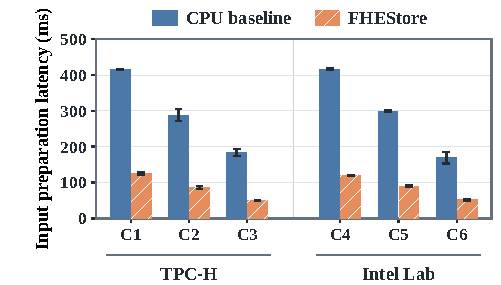
\includegraphics[width=\columnwidth]{figures/selective-generation/six-conditions.pdf}
  \caption{Input preparation under six application conditions, grouped by dataset. Error bars indicate sample standard deviations.}
  \Description{Grouped bars compare CPU baseline and FHEStore input preparation latency under conditions C1 through C6. TPC-H uses C1 through C3; Intel Lab uses C4 through C6. The conditions and encrypted output fields are defined in the accompanying table. FHEStore has lower mean latency in all six configurations.}
  \label{fig:selective-input-preparation}
\end{figure}

Figure~\ref{fig:selective-input-preparation} groups the six conditions by dataset. FHEStore reduces input-preparation latency in every configuration, achieving $3.29\times$--$3.65\times$ speedups over the CPU baseline. For the composite predicate C3 on TPC-H, time decreases from 183.92~ms to 50.38~ms; for C6 on Intel Lab, it decreases from 168.62~ms to 51.23~ms, corresponding to speedups of $3.65\times$ and $3.29\times$, respectively.
\bodypar

Changing the selected value range also changes the encryption workload. When target selectivity decreases from 75\% to 50\%, FHEStore input-preparation latency decreases from 124.54~ms to 85.90~ms for TPC-H and from 120.78~ms to 90.15~ms for Intel Lab. These results demonstrate application-directed input preparation across different selection conditions and output fields, using operator stream composition to connect preprocessing and encryption.
\bodypar

\subsection{Homomorphic Computation Correctness}
\label{sec:hpu-correctness}
We verify that ciphertexts generated by FHEStore support correct HPU homomorphic computation. The experiments cover bitwise OR, bitwise AND, equality, right shift, addition, subtraction, and multiplication, with plaintext sizes of 64, 128, 256, 512, and 1024 bytes per operand.
\bodypar

For the plaintext operands corresponding to each ciphertext batch, the host performs the same operation to generate reference results. After HPU computation, the host recovers the returned results using the corresponding key and compares the complete result sequence element by element, while also checking the output count. Addition, subtraction, and multiplication use results modulo 256, matching unsigned 8-bit arithmetic semantics.
\bodypar

Table~\ref{tab:hpu-correctness} summarizes the reference rules and verification results, where $x$ and $y$ denote the plaintext operands. Each configuration has three valid runs, except multiplication at a plaintext size of 1024 bytes, which has two.
\bodypar

% Counts derive from logs/csd_hpu_{64,128,256,512,1024}_{formal,eq_sub}_20261006/summary.csv.
% Include only OR, AND, EQ, SHR, ADD, SUB, MUL; exclude the extra SHL runs at 64.
% These FHEStore-produced inputs are distinct from the CPU-produced 29-operation suite.
\begin{table}[!htbp]
  \centering
  \caption{HPU correctness checks for FHEStore-generated ciphertexts.}
  \label{tab:hpu-correctness}
  \small
  \setlength{\tabcolsep}{3pt}
  \renewcommand{\arraystretch}{1.16}
  \begin{tabular*}{\columnwidth}{@{\extracolsep{\fill}}llr@{}}
    \toprule
    \textbf{Operation} & \textbf{Plaintext reference} & \textbf{Passed / Valid} \\
    \midrule
    OR & $x\mathbin{\mathrm{OR}}y$ & 15 / 15 \\
    AND & $x\mathbin{\mathrm{AND}}y$ & 15 / 15 \\
    EQ & 1 if $x=y$, otherwise 0 & 15 / 15 \\
    SHR & $x \gg (y\bmod 8)$ & 15 / 15 \\
    ADD & $(x+y)\bmod 256$ & 15 / 15 \\
    SUB & $(x-y)\bmod 256$ & 15 / 15 \\
    MUL & $(x\times y)\bmod 256$ & 14 / 14 \\
    \midrule
    Total & 35 configurations & 104 / 104 \\
    \bottomrule
  \end{tabular*}
\end{table}

All 104 valid correctness runs match the host reference counts and element-wise values, confirming that FHEStore prepares compatible ciphertext inputs for HPU homomorphic computation.
\bodypar

\section{Related Work}
\label{sec:related}
\noindent\textbf{Homomorphic Computation Acceleration.}
FHE accelerators improve homomorphic computation through specialized arithmetic and memory organization~\cite{xu2026hera,zhou2023fhemem,kim2022bts,kim2022ark}. F1 and CraterLake coordinate vector execution with data movement~\cite{samardzic2021f1,samardzic2022craterlake}, while FPT, MATCHA, and Strix optimize TFHE bootstrapping~\cite{vanbeirendonck2023fpt,jiang2022matcha,putra2023strix}. These designs accelerate the ciphertext consumer. FHEStore addresses the complementary input-preparation stage, coordinating persistent-data access, encoding, encryption, and ciphertext organization.
\bodypar

\noindent\textbf{Encryption and Client Processing.}
FPGA encryption engines have been developed for Brakerski/Fan--Vercauteren (BFV) and Cheon--Kim--Kim--Song (CKKS)~\cite{mert2020bfv,lee2023ckks}, as well as LWE and torus-based RLWE~\cite{feryputri2025lwe,syafalni2026multicore}. Client-side systems further explore encoding, memory organization, and communication around cryptographic processing~\cite{krieger2024aloha,yune2025abcfhe,vanderhagen2022choco,gupta2024memfhe}. FHEStore couples this processing to persistent-data access. Its HLS encryption operator integrates radix encoding with TFHE encryption and directs each generated mask coefficient to both dot-product accumulation and incremental ciphertext output.
\bodypar

\noindent\textbf{Computational Storage.}
Computational storage systems connect persistent data to programmable processing. Ibex offloads selection, projection, and aggregation~\cite{woods2014ibex}, and Biscuit composes host and device tasks through ordered data ports~\cite{gu2016biscuit}. INSIDER and DONGLE 2.0 provide programmable interfaces for data access and FPGA execution~\cite{ruan2019insider,wong2024dongle}. FHEStore's operator stream composition method connects optional preprocessing to encryption and accounts for ciphertext expansion through value-count-based buffer allocation and stream flow control.
\bodypar

\noindent\textbf{Storage-Coupled FHE Evaluation.}
Storage-coupled FHE designs integrate storage access with homomorphic evaluation~\cite{ohba2025nvme,suzuki2023isc}. Ohba et al. convey ciphertexts, keys, and programs through NVMe to an FPGA TFHE accelerator, while Suzuki and Yamana study CSD-coupled homomorphic execution. FHEStore's input-preparation task starts from persistent plaintext and supplies input ciphertexts to an external consumer.

\section{Conclusion}
\label{sec:conclusion}
FHEStore is an FPGA-based computational storage framework for FHE input preparation from persistent data. Its HLS encryption operator integrates radix encoding with TFHE encryption, sharing each mask coefficient between dot-product accumulation and incremental ciphertext output. The operator stream composition method connects optional preprocessing to encryption, determines buffer capacity from the value count and ciphertext representation, and coordinates execution through stream flow control. With 1~KiB of plaintext input, the encryption operator and input preparation achieve $5.00\times$ and $2.45\times$ speedups over the corresponding host CPU baselines, with lower cumulative host CPU time and peak host memory. The prepared ciphertexts support correct HPU homomorphic computation.

% Do not expose acknowledgments or identifying grant information in review.
% Add this environment, with real content, in the accepted version.
% \begin{acks}
% Acknowledge funding and assistance here.
% \end{acks}

\bibliographystyle{ACM-Reference-Format}
\bibliography{FHEStore_refs}

\end{document}
